
En el trabajo \cite{linsley1975fluctuation} se estudian los límites de confianza para la amplitud $r_1$ y la fase $\phi$ obtenidos mediante el análisis del primer armónico en Fourier. Las distribuciones de probabilidad describen a un conjunto de N mediciones cuya modulación en ascensión recta está caracterizada por el vector $\vec{s}$ con una dispersión $\sigma = \sqrt{\nicefrac{2}{N}}$.  Sin pérdida de generalidad, se puede restar a las mediciones la fase $\phi$ para que las mismas varíen alrededor del 0. Este vector $\vec{s}$ puede ser estimado mediante distintos métodos, en este trabajo se  utilizó como estimador el valor de la amplitud de la modulación en ascensión recta $r_1$ obtenido mediante el método de Rayleigh e East - West.

La distribución de probabilidad de la amplitud y la fase está dada por la Ec.\ref{eq:full_pdf}. Las variables $r$ y $\psi$ representan las amplitudes y fases medidas respectivamente
\begin{equation}
    p(r,\psi) =dr\,d\psi\,\frac{r}{2\pi\sigma^2}\exp{ -\frac{(r^2+s^2 - 2rs\cos\psi)}{2\sigma^2} } \label{eq:full_pdf}
\end{equation}  

\section{Distribución de probabilidad de la amplitud}

Integrando la Ec.\ref{eq:full_pdf} con respecto a $\psi$, se obtiene la función de densidad de probabilidad $p(r)$ y el nivel de confianza $CL$ entre en rango $[r_i,r_f]$:
\begin{align}
    p(r) &=\frac{r}{\sigma^2}\exp{ -\frac{(r^2+s^2)}{2\sigma^2} }K_0(\frac{rs}{\sigma^2})    \label{ec:pdf}\\
    CL_r(r_i,r_f,s) &= \int_{r_i}^{r_f} dr \, p(r)
    \label{ec:integral}
\end{align}
donde $K_0(x)$ es la función de Bessel modificada de primer orden.
Estas ecuaciones nos permiten determinar el nivel de confianza $CL$ con el cual se puede afirmar que el módulo del dipolo se encuentra entre los valores $r_i$ y $r_f$.

Se define el valor $r^{UL}$ como el límite superior donde se puede afirmar que el módulo de dipolo se encuentra en el rango $[0, r^{UL}]$ con un $99\%$ de certeza.
\begin{align}
    CL_r(0,r^{UL},s) = 0.99 = \int_{0}^{r^{UL}} dr \, p(r)
    \label{ec:r_upper_limit}
\end{align} 
% Para alcanzar un  nivel del confianza  del  CL[\%] \footnote{ Donde CL=.99 para un 99\% o CL=0.68 para un 68\%,},  se toma el valor de amplitud $r^{UL}$ y la integral de la función \ref{ec:pdf} desde 0 hasta $r^{UL}$, donde el resultado debe ser el nivel de confianza CL.
% \begin{align}
%     CL = \int_{0}^{r^{UL}} dr \frac{r}{\sigma^2}\exp{\Big( -\frac{(r^2+s^2)}{2\sigma^2} + \frac{rs}{\sigma^2}\Big)}K_0(\frac{rs}{\sigma^2})
%     \label{ec:integral}
% \end{align}

Suponiendo que mediante el análisis de un conjunto de eventos, se obtiene que $s=0.0047$ y $\sigma=0.0038$. El gráfico de la función $p(r)$ se muestra a continuación:

\begin{figure}[H]
    \begin{small}
        \begin{center}
            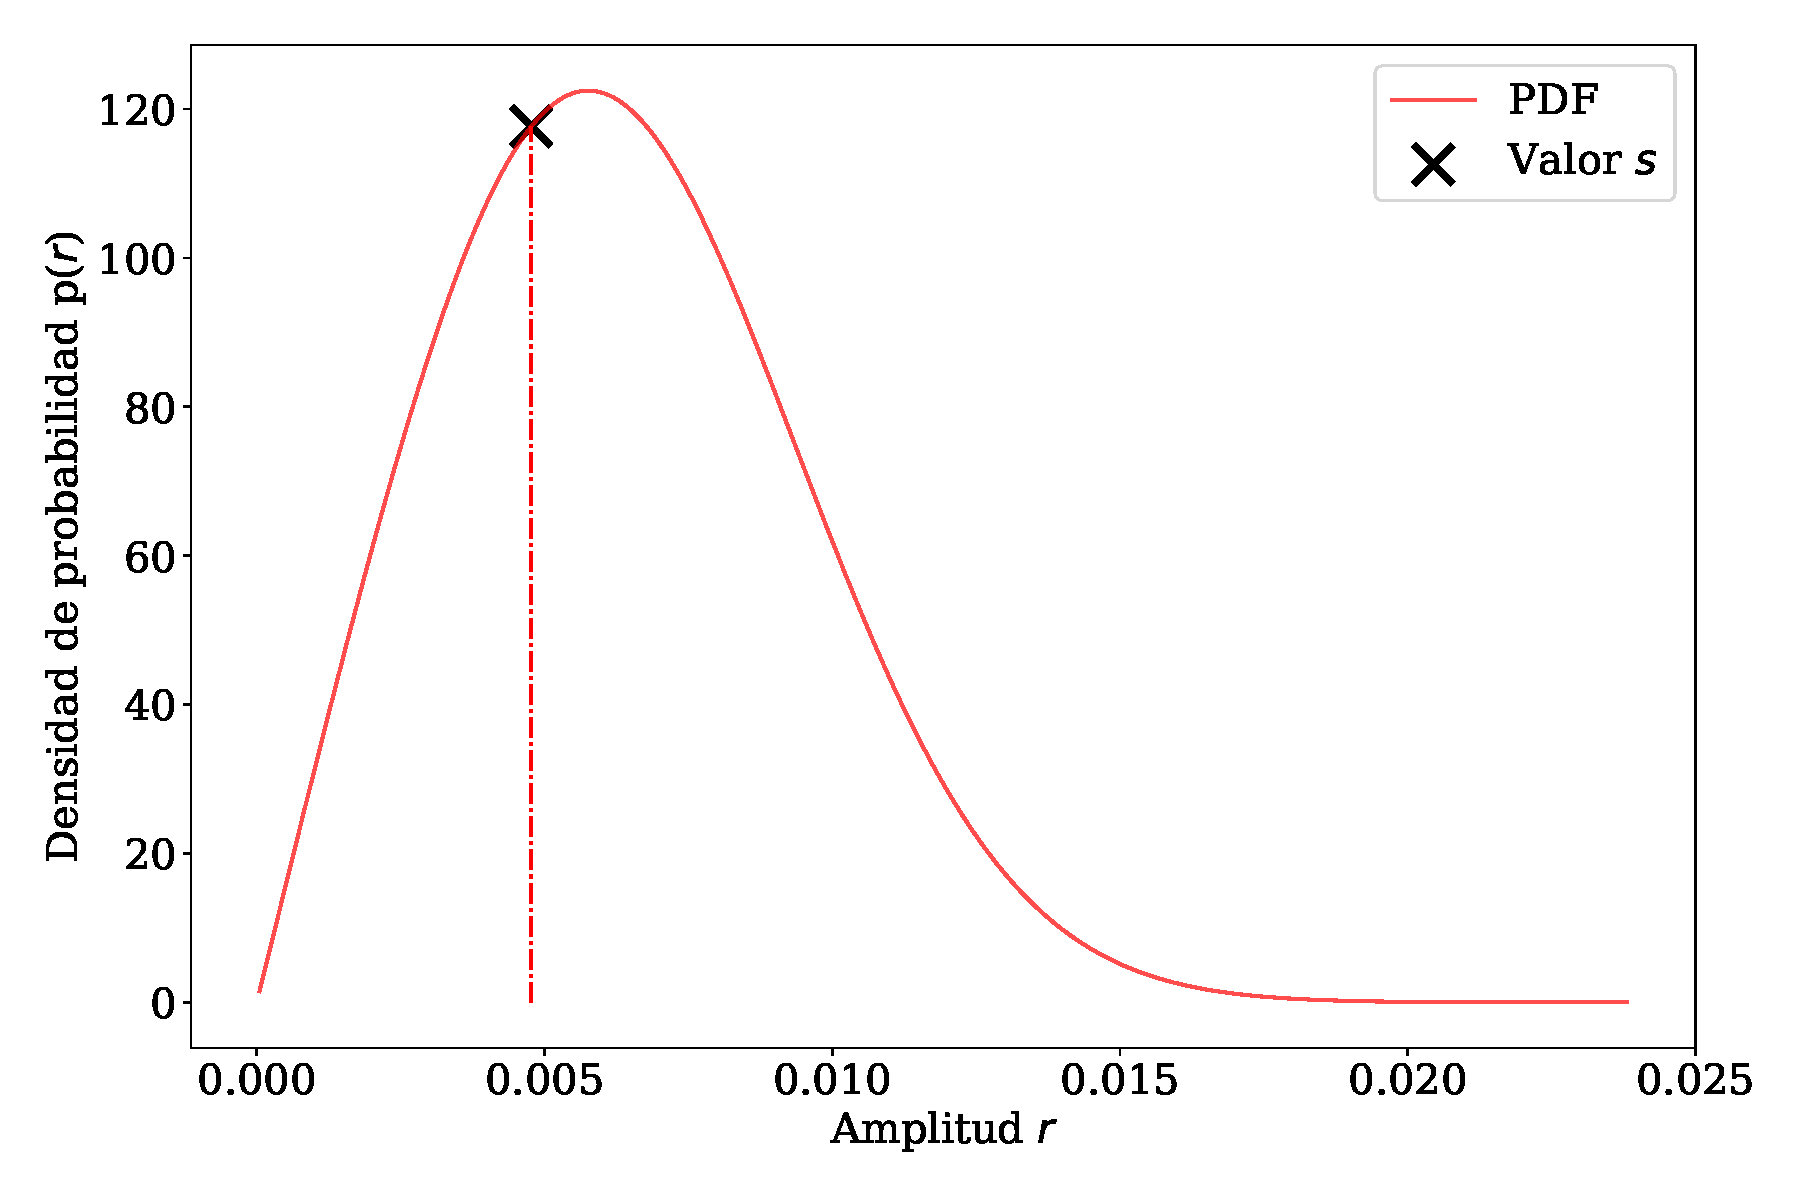
\includegraphics[width=0.75\textwidth]{bessel_prob_value_s_v2.pdf}
        \end{center}
        \caption{El gráfico de la densidad de probabilidad $p(r)$ de la amplitud $r$ para $s=0.0047$ y $\sigma=0.0038$ }
    \end{small}
\end{figure}

\subsection{Haciendo la cuenta de los márgenes de confianza de la amplitud}

Calculemos los márgenes de confianza para el ejemplo anterior de $s=0.0047$ y $\sigma=0.0038$. En este trabajo los márgenes que se obtuvieron nos dicen que el nivel de confianza en ese intervalo del $68.27\%$. Se toma este límite, dado que si $N>>1$, la distribución $p(r)$ tiende a una distribución normal y el nivel de confianza sería $1\sigma$.

Los pasos para el cálculo son los siguientes: 

\begin{enumerate}
    \item 
    Dado que la distribución tiene una función de bessel modificada de primer orden que diverge en el 0, se toma una aproximación a la función con los primeros 8 términos de la sucesión. Por lo que la función no es exacta y la norma difiere de $1$. 
    
    Para normalizar el área, se calcula la integral hasta $r_{max}=s +  10\sigma$, dado que está tan alejada del valor de amplitud obtenida, el nivel de confianza en $CL_r(0,r_{max},s)\simeq 1$, por lo que se  usa este valor para normalizar la Ec. \ref{ec:pdf} en el código.

    \item Una vez que se tiene la función normalizada, se calcula la integral de la ecuación \ref{ec:integral} $CL_r(0,s,s)$ en el intervalo  $[0,s]$ y se obtiene el valor de la función $p(s)=p_1$.

    % \item Si $CL_r(0,s,s)< 0.6827$:
    % \begin{enumerate}
        \item Teniendo en cuenta el valor inicial de $p_1$, se actualiza el valor  $p_2 \leftarrow p_1 - 0.01 p_1$ \label{itm:1}.
        \item Se calcula la integral entre los dos puntos con valores igual a $p_2$. 
        \item \label{itm:3} Si la integral es menor a $0.6827$, se repite el proceso desde el paso \ref{itm:1}. Caso contrario, si esta integral es mayor o igual a $0.6827$, se calculan los valores límites de $r$ mediante el valor $p_2$ en el paso \ref{pasofinal}. 

        La Fig.\ref{fig:itera} se muestra el área calculada en la primera iteración que se muestra verde, el valor de área obtenido no es el nivel de confianza buscada se sigue iterando hasta alcanzar el valor $p_N$, donde la integral entre esos extremos es de $0.6827$.
        \begin{figure}[H]
            \begin{small}
                \begin{center}
                    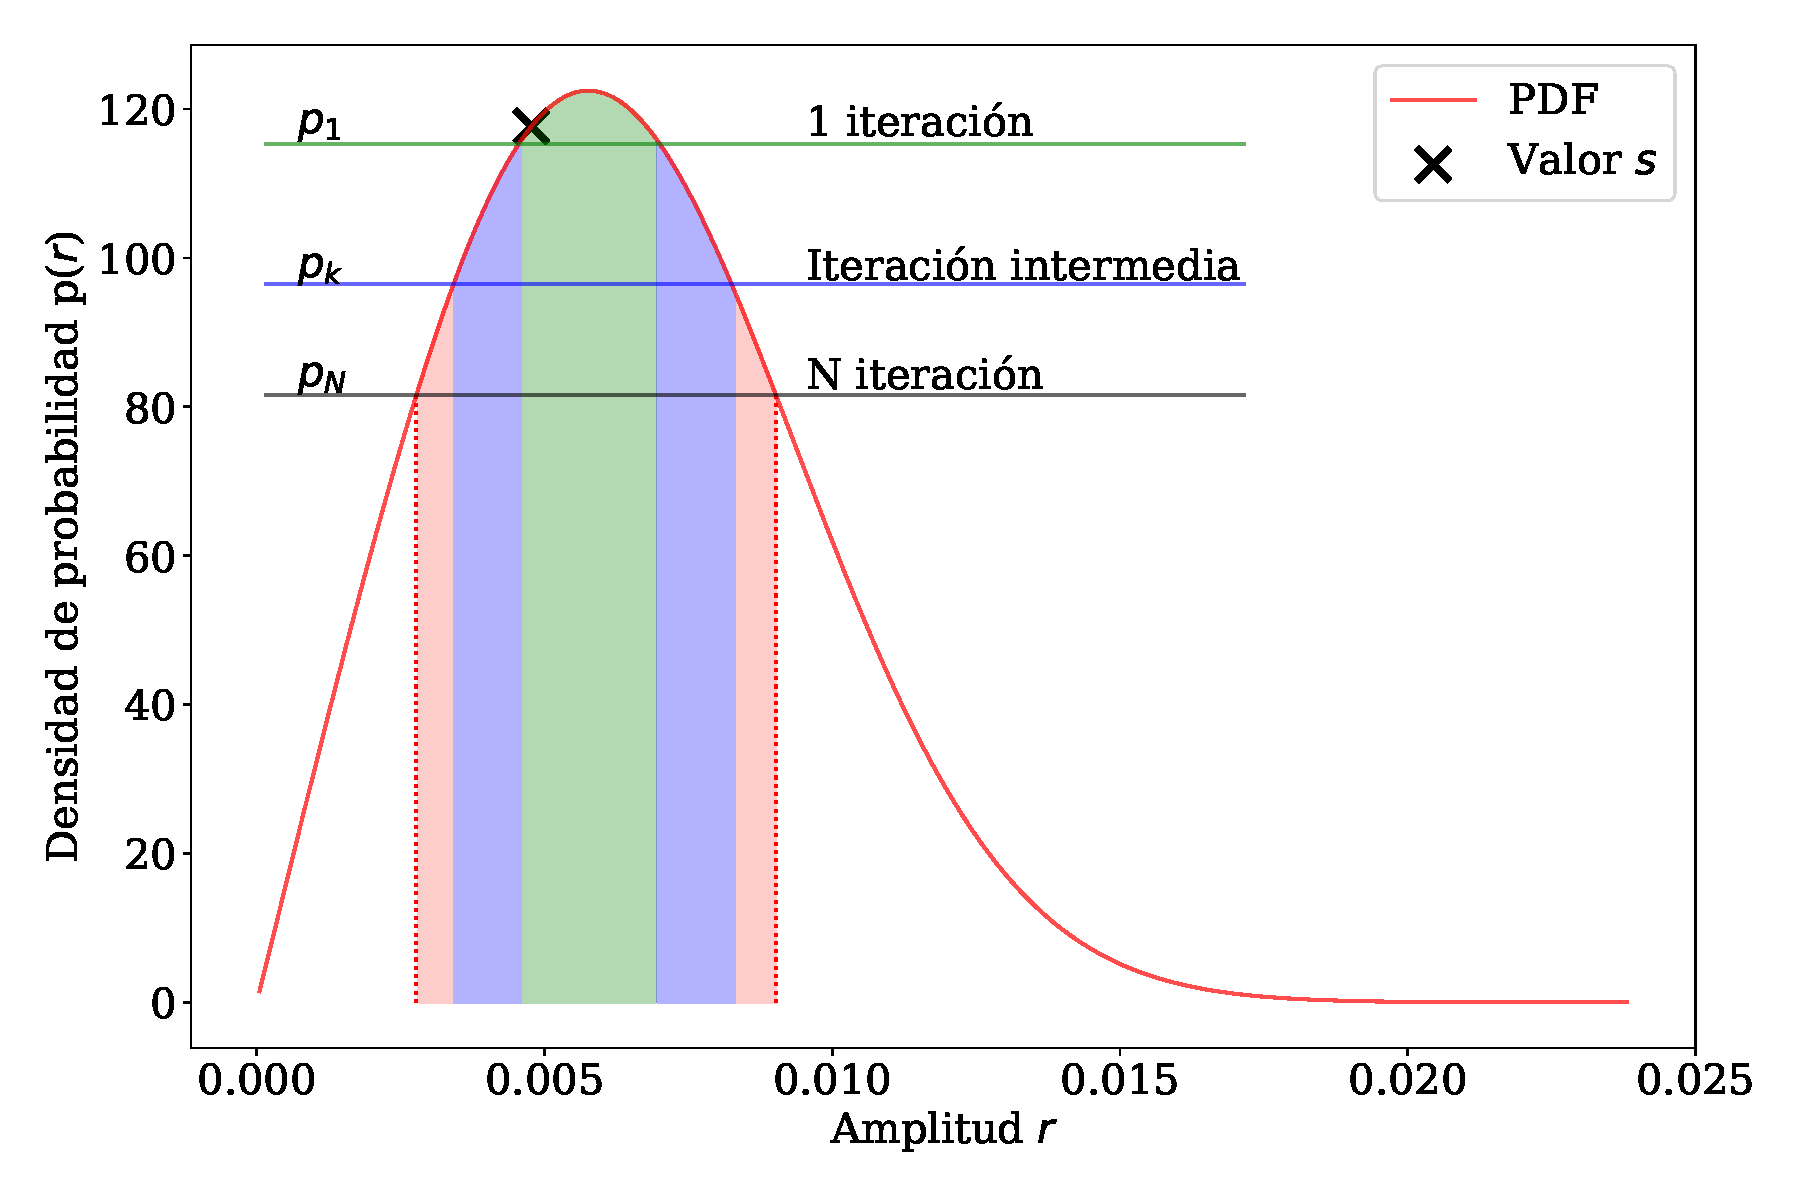
\includegraphics[width=0.75\textwidth]{bessel_prob_iterations_v2.pdf}
                \end{center}
                \caption{Iteraciones para encontrar los márgenes de confianza del $68.27\%$ de la distribución de probabilidad de la amplitud. En la N-ésima iteración se obtiene los límite de confianza buscados.}
                \label{fig:itera}
            \end{small}
            
        \end{figure}
    % \end{enumerate}
    \item Puede ocurrir que el valor de $s$ no esté entre los márgenes
     de confianza que se calcula. En este caso se toma como límite inferior $r^-$el valor $s$ y se busca el límite superior $r^+$ de tal forma que $CL(s,s+\sigma^+,s) \simeq 0.6827$.
    % \end{enumerate}
    \item \label{pasofinal} Los límites de confianza superior $r^+$  y inferior $r^-$, teniendo en cuenta el valor final $p_N$ del paso \ref{itm:3}, son tales que se cumple $p(r^+)=p(r^-)=p_N$. Finalmente los márgenes de confianza se calculan como:
    \begin{align*}
        \sigma^- = s-r^-\\
        \sigma^+ = r^+ -s
    \end{align*}
\end{enumerate}

En la Fig.\ref{margenes} se muestran los márgenes de confianza obtenidos para el ejemplo de $s=0.0047$ y $\sigma=0.0038$, el área sombreada es igual al $0.6827$
\begin{figure}[H]
    \begin{small}
        \begin{center}
            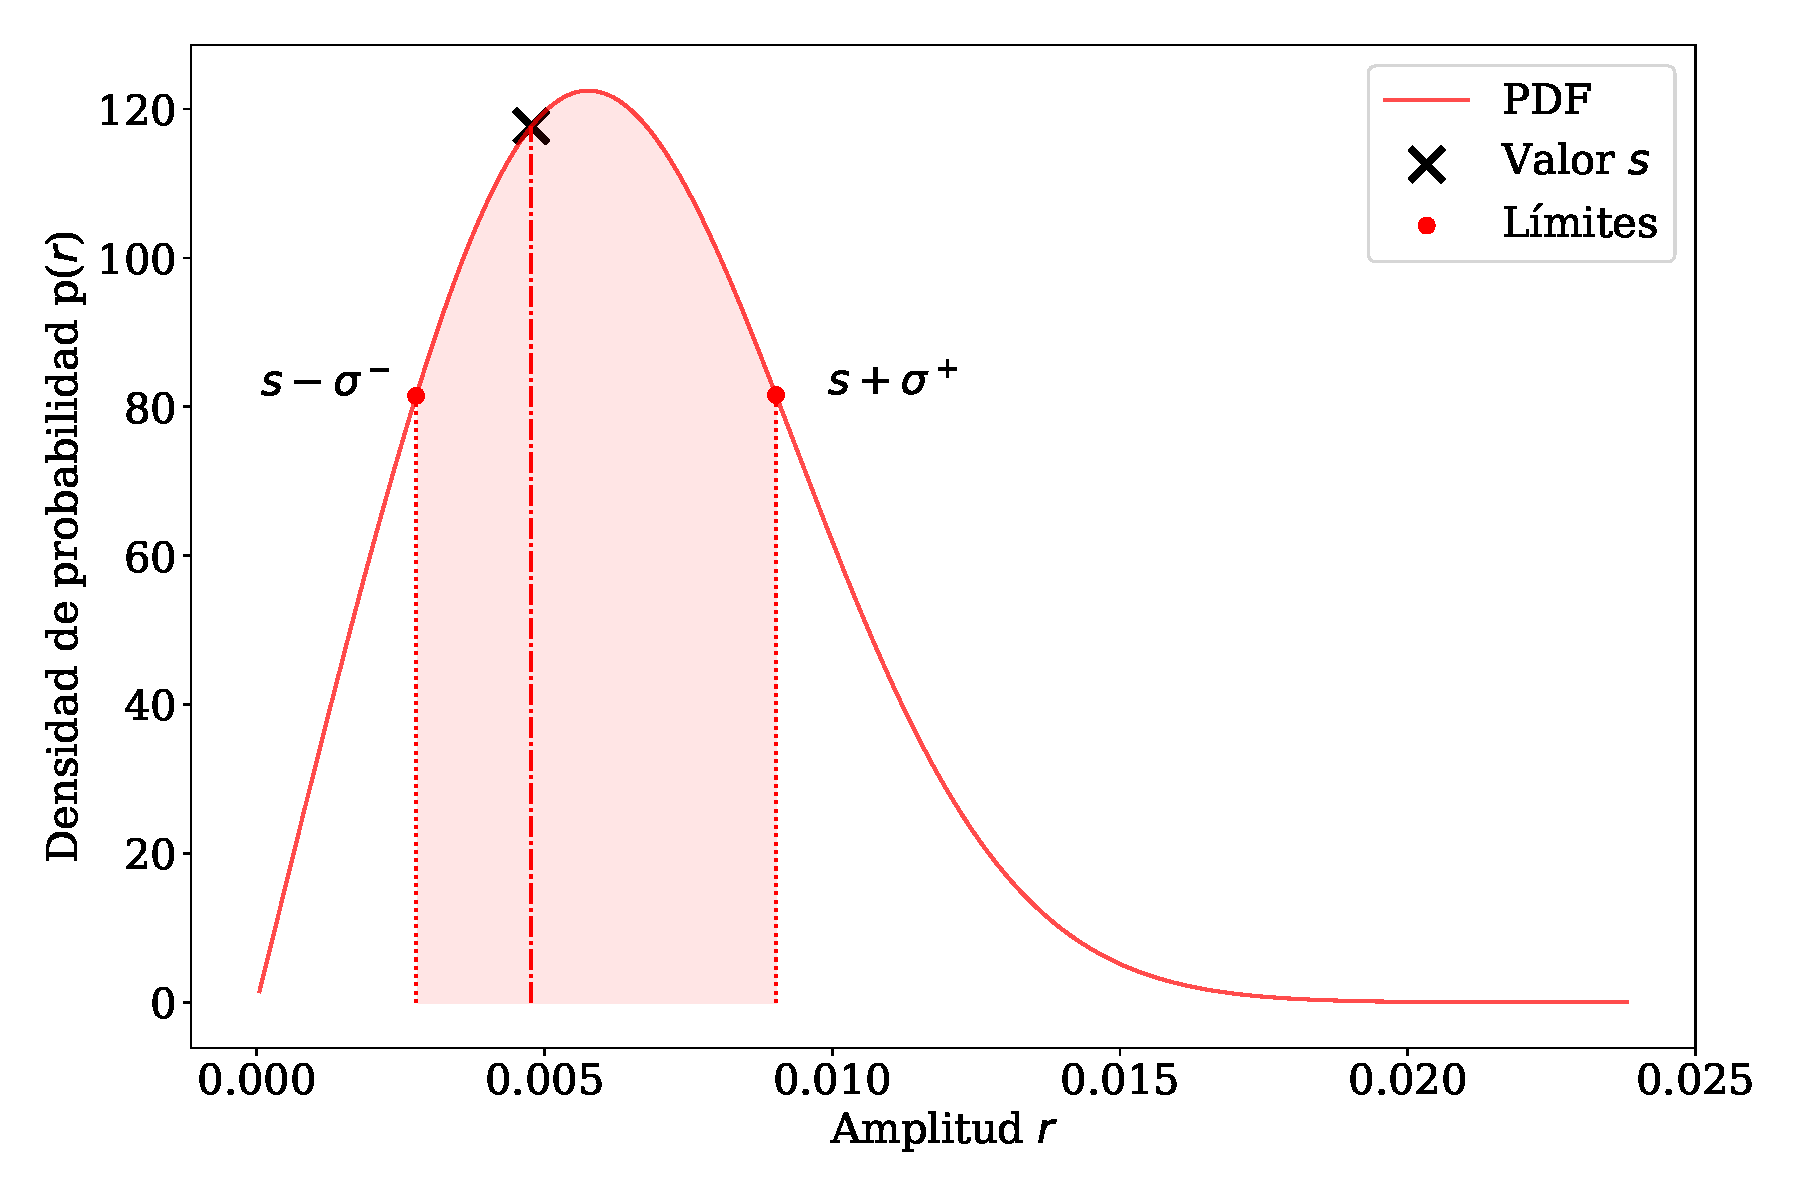
\includegraphics[width=0.75\textwidth]{bessel_prob_ej_v2.pdf}
        \end{center}
        \caption{Densidad de probabilidad de la amplitud $r$ para $s=0.0047$ y $\sigma=0.0038$. Se muestran los márgenes de confianza del $68.27\%$ }
        \label{margenes}
    \end{small}
\end{figure}

\section{Distribución de probabilidad de la fase del dipolo}

Integrando la ecuación \ref{eq:full_pdf} con respecto a $r$ en el rango $[0,\infty]$, se obtiene la distribución de probabilidad de la fase $\psi$ de la Ec.\ref{eq:phase_pdf}. Este apartado considera que las fases de la mediciones varían alrededor del cero. De esta forma, la distribución de probabilidad tiene la característica  de ser simétrica respecto a 0, por eso los límites de integración para obtener un nivel de confianza igual a 1 son $[-\pi, \pi]$.
\begin{align}
    p(\psi) &=d\psi\,\frac{1}{2\pi}e^{-k} \Bigg[ 1 + (\pi k)^{\nicefrac{1}{2}} \cos\psi e^{(k\cos^2\psi)} \Big( 1 + L \erf(L k^{\nicefrac{1}{2}} \cos\psi \Big) \Bigg ] \\ \label{eq:phase_pdf}
    CL_{\psi}(\phi_1, \phi_2, s) &= \int_{\phi_1}^{\phi_2} d\psi \, p(\psi)
\end{align}  
donde $k =\nicefrac{s^2}{2\sigma^2}$ y $\erf (x)$ es la función error, y
\begin{align*}
    L =
    \begin{cases} 
        +1 & \text{ Si } -\frac{\pi}{2} \leq x\geq \frac{\pi}{2} \\
        -1 & \text{ Caso contrario }  \\
     \end{cases}
\end{align*}

% La distribución de probabilidad tiene la característica  de ser simétrica respecto a 0, por eso los límites de integración son $[-\pi, \pi]$.

Se definió que el nivel de confianza para la fase reportada en este trabajo sea del $68.27\%$, ya que $k>>1$ la distribución de la fase se acerca a una distribución normal y este nivel de confianza es equivalente a $1\sigma_\phi$. 

Para calcular el margen de confianza $\sigma_\psi$,  dada la simetría de la función \ref{eq:phase_pdf}  con respecto al 0, se siguen los siguientes  pasos:

\begin{enumerate}
    \item Se toma un valor inicial de $\sigma_{\psi,0}=0.01$, que es equivalente a $0.57^o$.
    \item Se integra la Ec.\ref{eq:phase_pdf} en el rango $[-\sigma_{\psi,0}, \sigma_{\psi,0}]$ y se verifica si $CL_{\psi}(-\sigma_{\psi,0}, \sigma_{\psi,0},s) = 0.6827$.  Si ese es el caso, se reporta la fase como $\psi \pm \sigma_{\psi,0}$, caso contrario se vuelve al paso anterior con $\sigma_{\psi,1} \leftarrow \sigma_{\psi,0} + 0.01\sigma_{\psi,0}$. \label{paso2} y se itera hasta obtener el valor de $\sigma_{\psi,N}$ que cumpla $CL_{\psi}(-\sigma_{\psi,N}, \sigma_{\psi,N},s) = 0.6827$
\end{enumerate}

En la Fig.\ref{fig:phase_prob_ej} se muestra la distribución de probabilidad de la fase para $s=0.0047$ y $\sigma = 0.0038$, también se incluye los límites de confianza obtenidos.

\begin{figure}[H]
    \begin{small}
        \begin{center}
            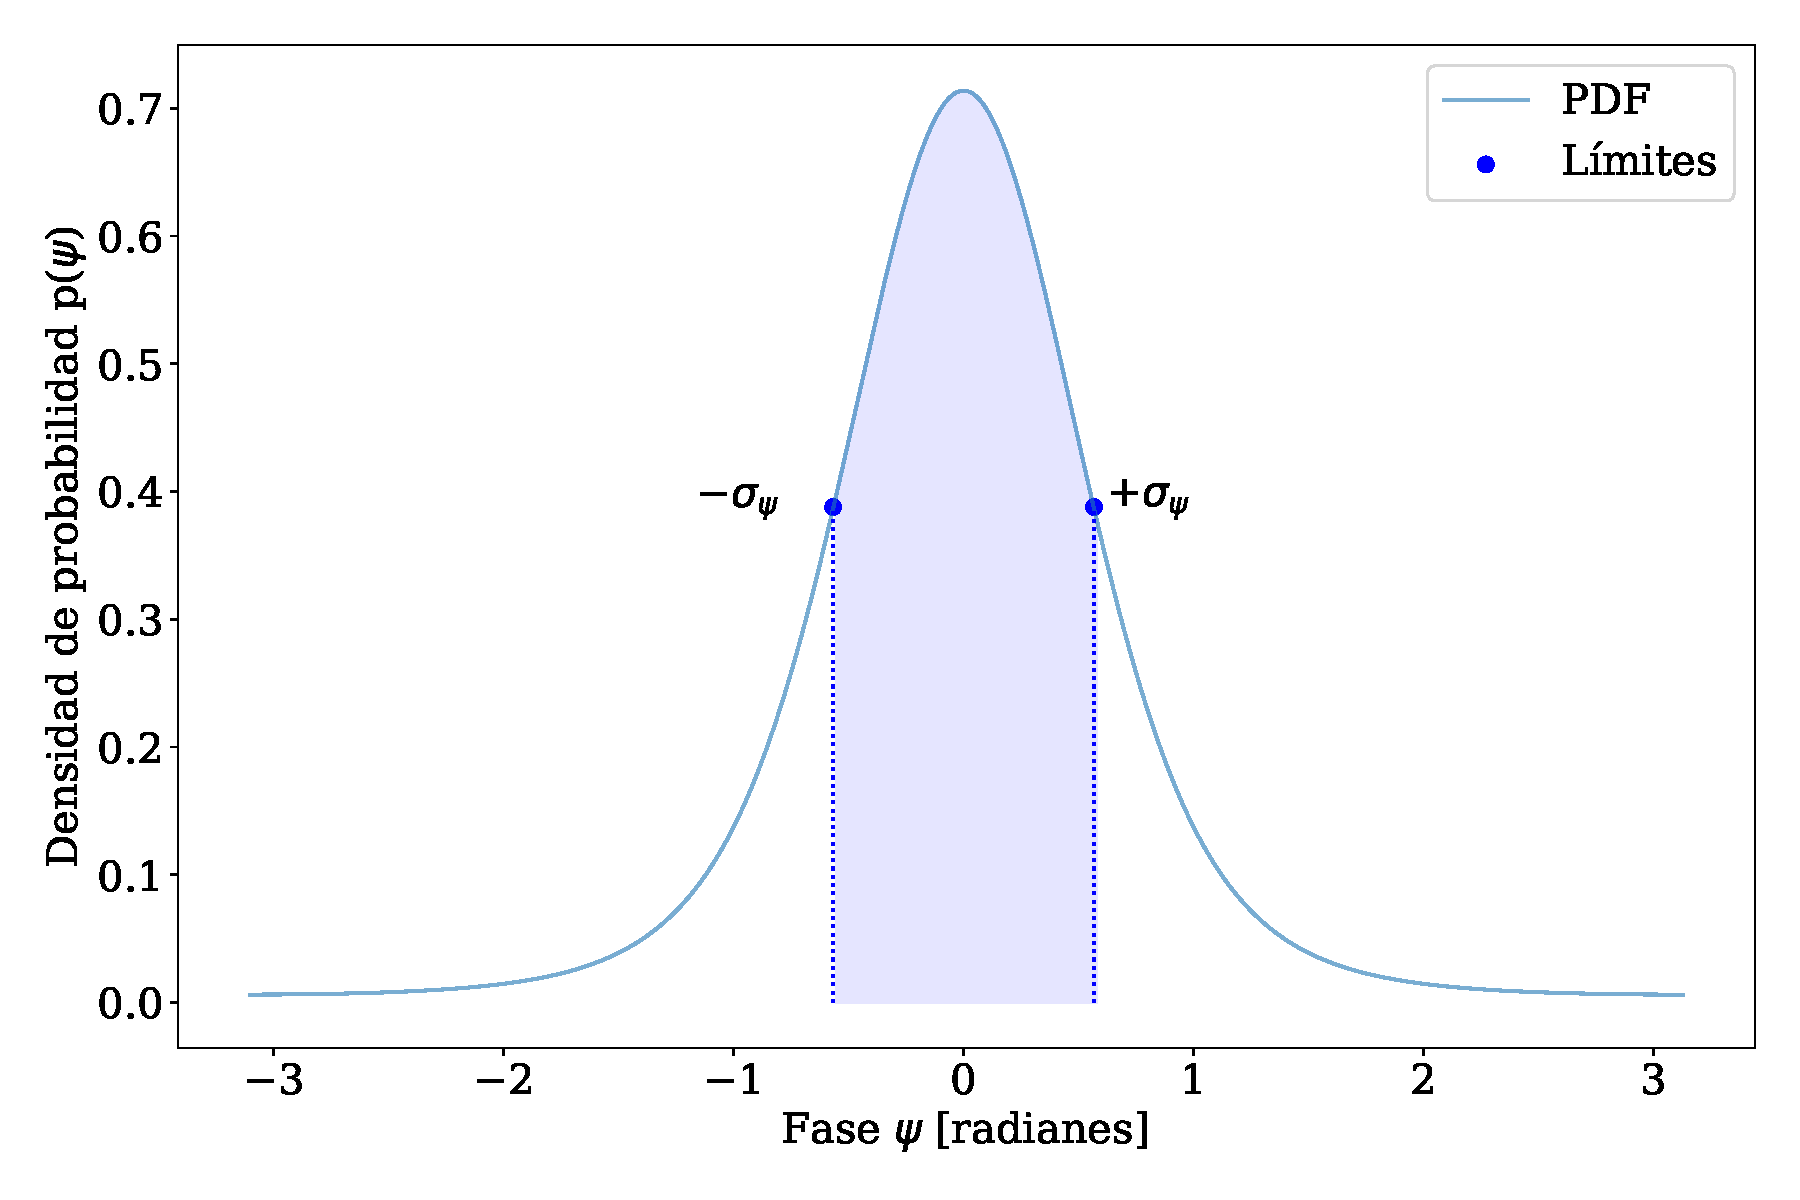
\includegraphics[width=0.75\textwidth]{phase_prob_ej_v2.pdf}
        \end{center}
        \caption{La distribución de probabilidad de la fase $\psi$ para $s=0.0047$ y $\sigma = 0.0038$ con los márgenes de confianza del $68.27\%$.}
        \label{fig:phase_prob_ej}
    \end{small}
\end{figure}